% Chapter on the conclusion.
%
% Developed for my Master Thesis at Maastricht University.
% Based on Eugenio Senes's template at the University of Torino.
%
% By Joeri Hermans (joeri@joerihermans.com)
%
% Released under an MIT license. Share, modify and enjoy, but quote the author!

\chapter{Conclusion}
\label{chapter:conclusion}

This work presents a detailed outline of the current landscape in distributed optimization with an application to Deep Learning. We started in Chapter~\ref{chapter:introduction} by giving a rough summary of different concepts, how they are currently applied, and their pitfalls. Furthermore, we introduced our first hypothesis, which states that \emph{workers optimize the central variable efficiently when they compute gradients based on older central variables which are close to the current central variable}, and was proved empirically on several occasions throughout this thesis.\\

In addition, while researching other distributed optimization methodologies, we found that \textsc{easgd}~\cite{zhang2015deep} and derivates, have very interesting properties. The first property, which is present in all \textsc{easgd} derrived algorithms, is the presence of an \emph{equilibrium} condition. Meaning, points exist during the optimization process that any additional computations done by a worker are inconsequential. Furthermore, this equilibrium is especially problematic if the central variable, and workers are close to a minima, causing \textsc{easgd} to converge (very) slowly to the minima. However, this equilibrium has desired side-effects in some cases, because it presents the optimizer from overfitting, as shown empirically in our experiments. Furthermore, a second interesting observation was that in the asynchronous version of \textsc{easgd}, i.e., \textsc{aeasgd}, the workers are not \emph{pushing} the central variable towards a minima, as is the case in settings similar to \textsc{downpour}. But the workers rather act as a normal distribution around the central variable, i.e., the central variable as the mean of the distribution, with the variance of the distribution being proportional to the exploration hyperparameter $\rho$. Afterwards, we considered \textsc{dynsgd}~\cite{jiang2017heterogeneity}, which is an attempt to deal with staleness in a non-\emph{stale-synchronous} manner. However, using our hypothesis, we showed that the way \textsc{dynsgd} deals with staleness, which is in terms of stale steps, is a rather naive approach.\\

This resulted in the next contribution of this thesis, \textsc{agn}, which is described in Chapter~\ref{chapter:accumulated_gradient_normalization}. During the development of \textsc{agn}, we made the same \emph{practical} assumptions with respect to constraints as \textsc{easgd}, i.e., high communication costs. However, it was desired that the optimizer did not have the equilibrium issues \textsc{easgd} derrived algorithms had. As a result, we turned to \textsc{downpour}, and allowed for more local exploration by sending \emph{accumulated gradients} to the parameter server. However, this approach diverged even quicker than regular \textsc{downpour}, with the difference that data was processed significantly faster due to the reduced waits. As a result, \textsc{agn} was adapted to use the time between parameter updates more efficiently by computing a \emph{better} gradient based on a normalized sequence of first-order gradients. Furthermore, we showed that \textsc{agn} outperforms all currently existing distributed optimizers in terms of training, and validation accuracy in the presence of a large amount of concurrency and reduced communication frequency. However, since \emph{stability} is also important in distributed optimization, we introduced a new metric called \emph{temporal efficiency}, which basically is the ratio between the integrated area of training metrics of two difference optimizers. As a result, not only the final training accuracy is considered, but also the stability, and time it took to reach that accuracy.\\

In addition, as the number of asynchronous workers was increased in \textsc{agn}, divergent behaviour started to occur. However, \textsc{agn} was able to stabilize in all situations. Nevertheless, this behaviour is not desired, as it impairs the convergence rate of the central variable. To combat this issue, \emph{staleness} had to be redefined in Chapter~\ref{chapter:asynchronous_distributed_adaptive_gradients}. Contrary to the old definition of staleness (in terms of stale steps), staleness in parameterized settings is defined as the distance between the parameterization of the central variable on which a worker bases its gradients, and the current parameterization of the central variable. This new definition of staleness, together with \emph{implicit momentum}~\cite{implicitmomentum}, shows why other asynchronous optimizers tend to divergence when committing accumulated gradient, or by simply increasing the number of workers. Furthermore, it also shows why \textsc{dynsgd} had troubles converging, since what really matters is not the stale steps, but rather the magnitude of the gradient updates. Using this novel intuition, we constructed a new mechanism to deal with staleness, and further improve the stability of distributed optimizers. The mechanism, \textsc{adag}, can in principle be combined with any distributed optimization procedure. However, to efficiently compute the per-weight scaling factor, one needs to consider the Algorithms described in Chapter~\ref{chapter:asynchronous_distributed_adaptive_gradients}, and evaluate their pros and cons.\\

Finally, we introduced and described the experimental setup~\cite{dist_keras} in Chapter~\ref{chapter:experiments}. We constructed the experimental framework, \emph{dist-keras}, to serve several purposes. However, the main focus of this framework is on distributed optimization. To accomplish this, the programming interface was simplified with the purpose to easily implement new distributed optimizers. In addition, since validation and other training metrics can be computed on different nodes in parallel with ease, because of the provided utility classes, a better statistic of a model can be obtained by simply increasing the amount of validation data.

\section{Contributions}
\label{sec:conclusion_contributions}

This Section summarizes the contributions of this work, and their empirical validation. First, we examined existing distributed optimization algorithms such as \textsc{downpour}~\cite{dean2012large}, \textsc{easgd}~\cite{zhang2015deep}, and \textsc{dynsgd}~\cite{jiang2017heterogeneity}. As previously shown, we validate the result that \textsc{downpour}~\cite{dean2012large} becomes very unstable as the number of parallel workers increases~\cite{implicitmomentum, hadjis2016omnivore}. To combat this, and to solve the communication constraints,~\cite{zhang2015deep} proposes \textsc{(a)easgd}. Again, we validate the claim of the authors that \textsc{aeasgd} performs better when a low communication frequency is used. However, we showed in Chapter~\ref{chapter:distributed_deep_learning} that due to the \emph{elastic difference} mechanism an equilibrium condition occurs which impairs the convergence rate of \textsc{(a)easgd}, shown in Figure~\ref{fig:conclusion_equilibrium_early_stopping}. Furthermore, when \textsc{(a)easgd} approaches an equilibrium, additional local computations are in essence \emph{wasted}, since they won't push the equilibrium boundary any further because the elastic difference between the worker and the central variable is too large, i.e., worker and central variable are too distant. As a result, one could prevent the waste of computational resources by implementing an \emph{early stopping} mechanism whenever a worker approaches an equilibrium condition. This means whenever Equation~\ref{eq:easgd_equilibrium_fix} is satisfied, or when the communication frequency of the worker is expired, the elastic difference is communicated with the parameter server. This has the desired effect that the convergence rate of the central variable is drastically improved, given the fact that the network and the implementation is able to handle the increased bandwith consumption.\\

The second main contribution of this thesis is an attempt to solve the \emph{wasting} of computational resources in \textsc{(a)easgd} due to the equilibrium condition described above. We do this by adapting \textsc{downpour} to perform gradient accumulation (exploration), and apply a normalization factor which is proportional to the amount of local exploration steps that needs to be done ($\lambda$). As shown in Chapter~\ref{chapter:accumulated_gradient_normalization}, this results in a gradient update which is normalized with respect to the amount of local exploration steps. Meaning, whenever a worker computes a \emph{sequence} of $\lambda$ gradients, it will normalize (average) those gradients with $\lambda$. This will cause a gradient update to be reduced in magnitude, but, it will provide a better direction to a minima, and therefore is able to handle parameter staleness more efficiently. We call this technique \emph{Accumulated Gradient Normalization}, or in short, \textsc{agn}. Furthermore, we show that for most configurations \textsc{agn} outperforms \textsc{dynsgd} and \textsc{aeasgd} in terms of training accuracy, and thereby obtaining a state-of-the-art performance regarding distributed optimization using gradient-based methods.\\

However, as we increase the number of asynchronous workers in the optimizers discussed above, stability issues occur during the optimization process. This instability is caused by parameter staleness. An initial attempt to mitigate the staleness problem was to scale worker updates with respect to the number of stale steps~\cite{jiang2017heterogeneity}. However, as shown in Chapter~\ref{chapter:distributed_deep_learning}, this approach is quite naive and does not address the underlaying issue. In Chapter~\ref{chapter:asynchronous_distributed_adaptive_gradients}, we introduced a \emph{novel} definition of parameter staleness, and constructed a mechanism (\textsc{adag}) which uses this definition to deal with parameter staleness effectively contrary to existing methods. Furthermore, to compare different distributed optimization algorithms against each other in terms of convergence rate and stability, we introduced a novel metric called \emph{temporal efficiency}, described in Equation~\ref{eq:temporal_efficiency}. Summarized, the following main contributions are made in this thesis:

\begin{itemize}
\item Equilibrium condition of \textsc{(a)easgd}~\cite{zhang2015deep}, and early stopping mechanism to improve convergence rate of \textsc{(a)easgd}.
\item Redefinition of parameter staleness in terms of distance between two parameterizations.
\item Two novel mechanisms, \textsc{agn} and \textsc{adag}, with state-of-the-art performance and robustness against (distributed) hyperparameterization.
\item A novel evaluation metric, \emph{temporal efficiency}, which also takes the stability of the convergence into account, which is important in distributed optimization due to the presence of parameter staleness.
\item Asynchronous optimization really benifits close to an minima, since our definition of parameter staleness says that staleness is small.
\end{itemize}

\begin{figure}
  \centering
  \begin{subfigure}{.49\textwidth}
    \centering
    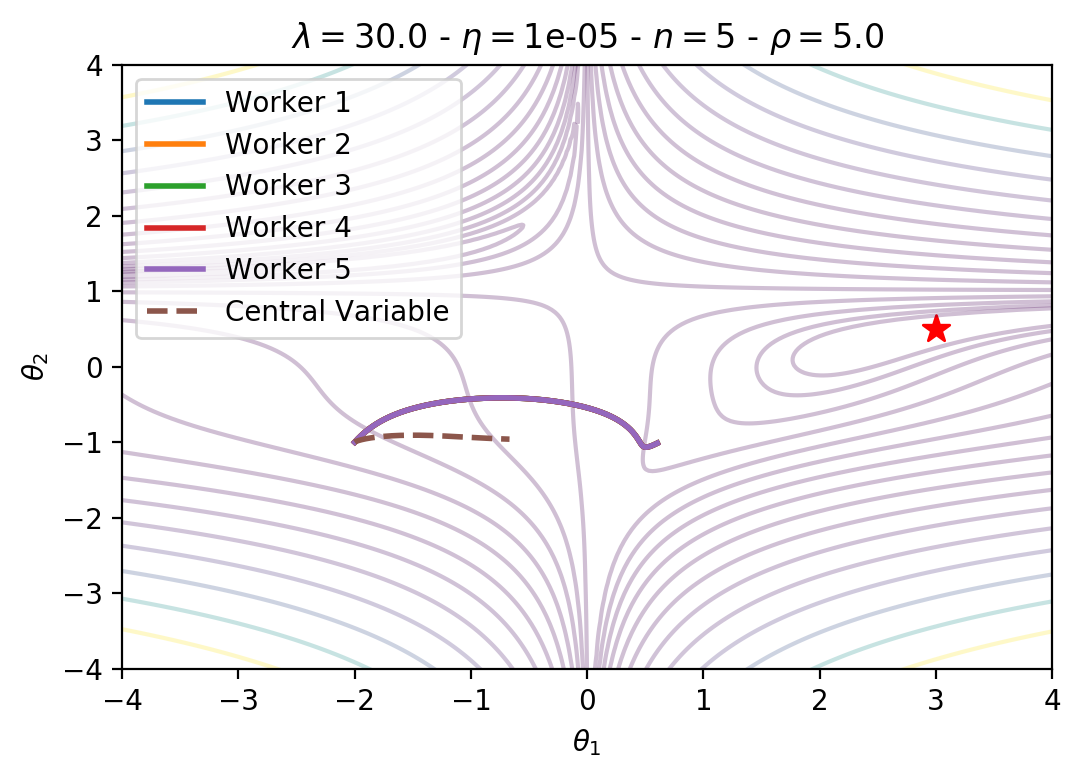
\includegraphics[width=\linewidth]{resources/images/easgd_sync_norm_space.png}
    \caption{Equilibrium, no early stopping.}
  \end{subfigure}
  \begin{subfigure}{.49\textwidth}
    \centering
    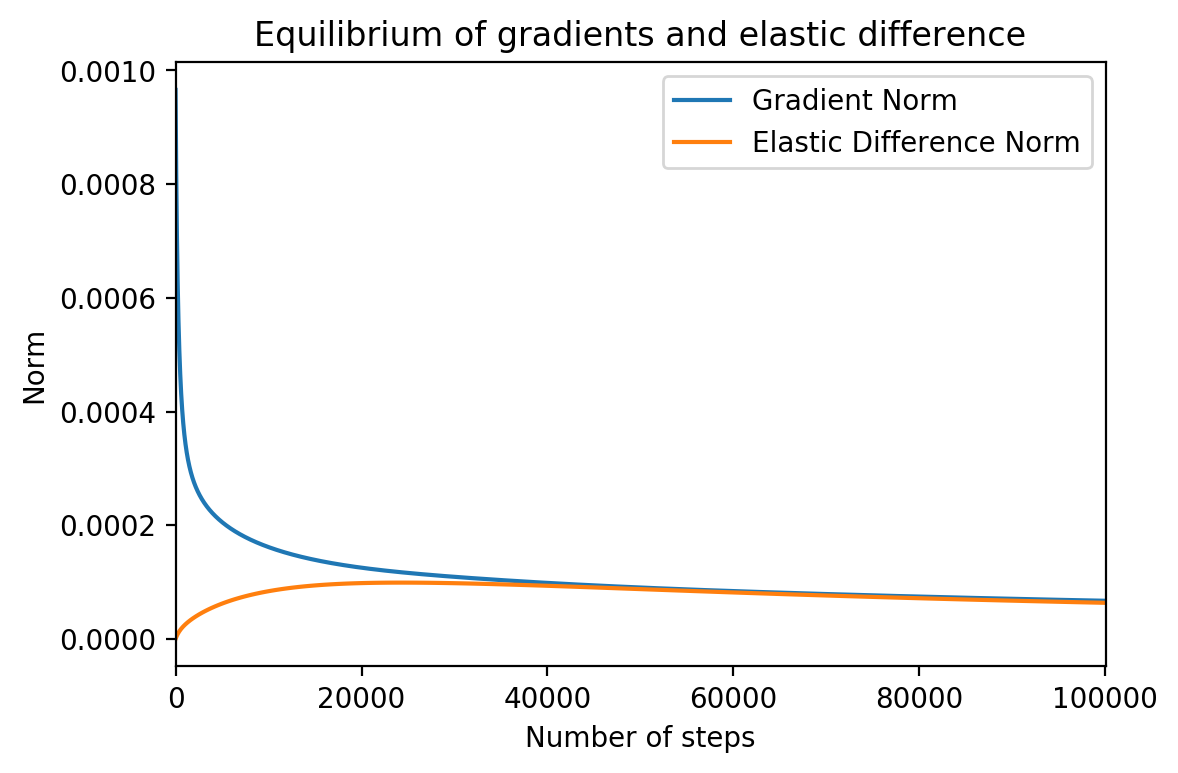
\includegraphics[width=\linewidth]{resources/images/easgd_sync_norm_equilibrium.png}
    \caption{Equilibrium, no early stopping.}
  \end{subfigure}
  \begin{subfigure}{.49\textwidth}
    \centering
    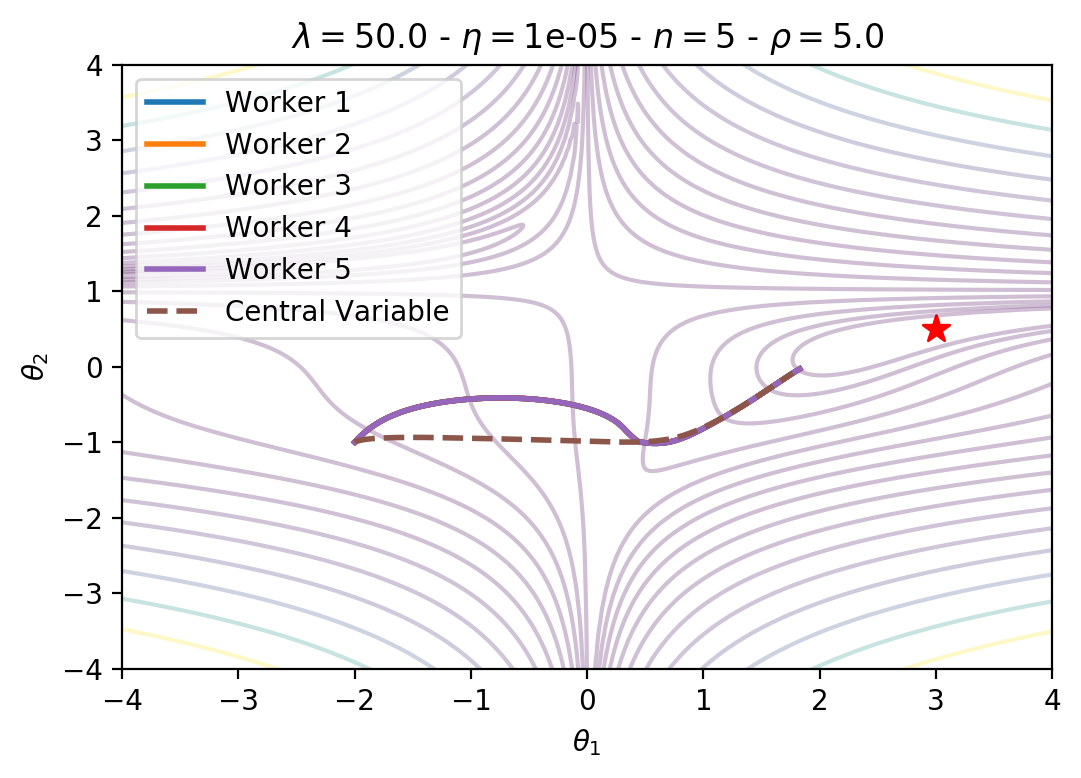
\includegraphics[width=\linewidth]{resources/images/easgd_es_50_y}
    \caption{Equilibrium, early stopping.}
  \end{subfigure}
  \begin{subfigure}{.49\textwidth}
    \centering
    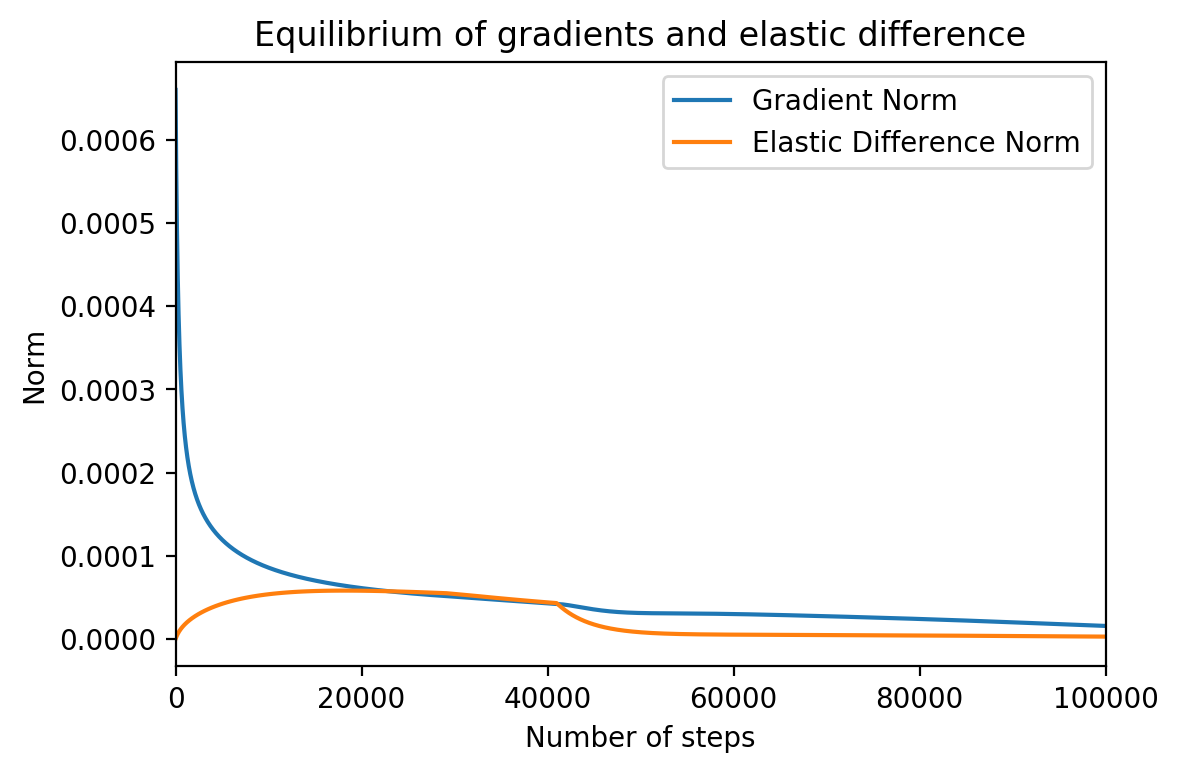
\includegraphics[width=\linewidth]{resources/images/easgd_es_50_y_eq}
    \caption{Equilibrium, early stopping.}
  \end{subfigure}
  \caption{Equilibrium condition of \textsc{(a)easgd} described in Section~\ref{sec:easgd}. To improve the convergence rate of \textsc{easgd}, we propose an early stopping mechanism which is triggered when a worker is approaching an equilibrium condition.}
  \label{fig:conclusion_equilibrium_early_stopping}
\end{figure}

\section{Research Questions}
\label{sec:conclusion_research_questions}

In Section~\ref{sec:problem_statement}, we posed several Research Questions which guided the work conducted in this thesis. Using the knowledge gained by researching this topic, those questions can now be answered.\\

\noindent \textbf{Research Question 1.}\\
\emph{When do workers contribute positively to the central variable during training?}\\

Using our new definition of staleness in parameterized settings, and the fact that \emph{implicit momentum}~\cite{implicitmomentum} follows from parameter staleness, a worker contribution is positive when the distance between the old central variable, which the worker used to compute its commit, and the current central variable is small. However, as shown in Chapter~\ref{chapter:accumulated_gradient_normalization}, staleness in terms of parameter distance is not really an issue if a better \emph{direction} to a minima is provided.\\

To deal with parameter staleness in a highly concurrent configuration, we introduced \textsc{adag} to construct a per-weight scaling factor which would scale a delta down proportional to the distance of the old, and new central variable. Which resulted in a more stable convergence rate of the central variable due to the automatic scaling of updates from stale workers. Furthermore, in the case that staleness becomes less of an issue over time, possibly due to the existence of a plateau or a minima, workers which were scaled significantly before due to staleness, will now contribute positively to the central variable. Thus, reaching the minima faster due to an \emph{implicit} increase in asynchrony.\\

\noindent \textbf{Research Question 2.}\\
\emph{Why does asynchronous \textsc{easgd} diverge when a small communication frequency is used, and converges with a large communication frequency?}\\

Using \emph{dist-keras}~\cite{dist_keras}, and even in simulations, we sometimes observed divergent behaviour of \textsc{aeasgd}. After several experiment, we concluded that this instability is induced by a numerical error when the difference between the old central variable, and current central variable is relatively large (stale). In addition, if an \textsc{aeasgd} worker commits a very stale \emph{elastic difference} to the parameter server, it causes other workers to be very stale as well because workers in \textsc{easgd} do not \emph{synchronize} with the central variable. Thus, causing the divergent behaviour. However, this could be corrected with \textsc{adag}, with the disadvantage of an increased computational cost.\\

\noindent \textbf{Research Question 3.}\\
\emph{What is the nature of staleness in parameterized settings?}\\

According to Definition~\ref{def:staleness}, staleness in parameterized settings can be defined as: \emph{Given a parameterization for worker $k$ at time $t$, $\theta^k_t$, based on the central variable $\tilde{\theta}_{t - \tau}$ where $\tau$ is the number of stale steps, and a central variable at time $t$, $\tilde{\theta}_t$. Then, staleness is defined as the difference (distance) between $\tilde{\theta}_t$ and $\tilde{\theta}_{t-\tau}$}.

\section{Future Work}
\label{sec:conclusion_future_work}

To conclude this thesis, several interesting points came up during this work that could be addressed in future work:\\

An initial point that could be addressed is to provide a better understanding how $\gamma$ should be defined in \textsc{adag}. A lower $\gamma$ is usually correlated with a higher amount of concurrency in the optimization procedure. Therefore it might be related to \emph{implicit momentum}, as on average, per time-unit, the central variable traversed a larger distance in the parameter space compared to a smaller amount of concurrent workers.\\

To further improve \textsc{adag}, and possibly reduce to computational complexity, we could take inspiration from the \emph{elastic difference} in \textsc{aeasgd}, and modify it in such a way that the term could be used to combat staleness in \textsc{agn}.\\

Practical and performant system architectures are also an important aspect that needs to be addressed to improve the convergence rate of a central variable. Therefore, some work has to be done to construct a performant system architecture which is able to deal with failures, and large datascales, i.e., peta- or even exabyte scale. Data scale is also an additional issue that is mostly forgotten about, or regarded as a \emph{technical} issue. For example, consider a multi-epoch training procedure on petabyte scale, do we congest the network by sending the training data multiple times over the network, or do we cache some locally? Furthermore, in most cases the data has to be reshaped into a format a model can work with. How do we accomplish this, do we transform the data on the fly (multiple epochs, network cost, computation cost), or do we transform all data once, and store them elsewhere (storage cost). However, to understand asynchronous gradient descent even better, working on such systems might provide additional insights that can be used to solve other issues in non-distributed settings, and even solve problems in computer engineering fields.
